\documentclass{beamer}
\usepackage[utf8]{inputenc}
\usepackage[T1]{fontenc}

\usebackgroundtemplate{
	
\includegraphics[width=\paperwidth,height=\paperheight]{img/background}
}

\title{Chapter 02: Entity-Relationship Modeling}

\author[P.A. Nugroho]{Pascal Alfadian Nugroho}
\institute[IF-UNPAR]{Program Studi Informatika, \\Universitas Katolik Parahyangan}

\begin{document}
	\begin{frame}
		\titlepage
	\end{frame}

	\section{Introduction}
	\begin{frame}{Introduction}
		\begin{itemize}
			\item Emphasis in structured system analysis is on the \textbf{operations}, rather than \textbf{data}
            \item Entity-relationship Modelling (ERM) is a semiformal data-oriented technique for specifying the product.
            \item Obviously, you can do both for analyzing projects.
		\end{itemize}
	\end{frame}
	\begin{frame}{Introduction}
		\begin{itemize}
			\item The modelling are mostly done using the Entity-Relationship Diagram (ERD)
			\item The benefit, is that it can be easily converted to SQL database tables
            \item Turns out there are so many variations in modelling, and very well described in \cite{song1995}
            \item In this lecture, we are using ``Visual Paradigm'' tool, which is based on Barker (a.k.a. CASE*) notation \cite{barker1992case}. The Community Edition is free.
		\end{itemize}
	\end{frame}
	
	\section{Basic Examples of ERD}
	\subsection{Simple Entity-Relationship Diagram}
	\begin{frame}{Simple Entity-Relationship Diagram}
		\begin{columns}[t,totalwidth=\textwidth]
			\column{.5\linewidth}
				\begin{itemize}
					\item This is a simple example of ERD, from \cite{Schach:2006:OCS:1207045}
					\item There, an entity ``Author'' is specified, denoted by a rectangle.
					\item One author can write many ``Novel'' entity, denoted by the line (one-to-many relationship).
					\item ``Reader'' has two one-to-many relationship to ``Novel``: reads and owns.
				\end{itemize}
			\column{.5\linewidth}
				\begin{flushright}
					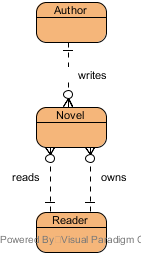
\includegraphics[scale=0.7]{img/02_simple_erd}
				\end{flushright}
		\end{columns}
	\end{frame}
	
	\section{Basic Examples of ERD}
	\subsection{Simple Entity-Relationship Diagram}
	\begin{frame}{Simple Entity-Relationship Diagram}
		\begin{columns}[t,totalwidth=\textwidth]
			\column{.7\linewidth}
    		    \begin{small}
                \begin{table}[]
                \centering
                \caption{``authors'' and ``readers''}
                \begin{tabular}{|l|l|l|}
                \hline
                \textbf{Name} & \textbf{Type} & \textbf{Extras} \\ \hline
                id            & INT(11)       & Primary Key     \\ \hline
                \end{tabular}
                \end{table}
                \begin{table}[]
                \centering
                \caption{``novels''}
                \begin{tabular}{|l|l|l|}
                \hline
                \textbf{Name}           & \textbf{Type} & \textbf{Extras}        \\ \hline
                id                      & INT(11)       & Primary Key            \\ \hline
                written\_by\_author\_id & INT(11)       & Foreign Key to authors \\ \hline
                read\_by\_reader\_id    & INT(11)       & Foreign Key to readers \\ \hline
                owned\_by\_reader\_id   & INT(11)       & Foreign Key to readers \\ \hline                
                \end{tabular}
                \end{table}
                \end{small}
			\column{.3\linewidth}
				\begin{flushright}
					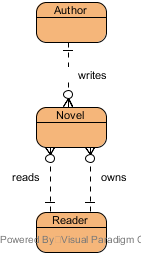
\includegraphics[scale=0.6]{img/02_simple_erd}
				\end{flushright}
		\end{columns}
	\end{frame}
	
	\subsection{Many-to-Many Entity-Relationship Diagram}
	\begin{frame}{Many-to-Many Entity-Relationship Diagram}
		\begin{columns}[t,totalwidth=\textwidth]
			\column{.5\linewidth}
				\begin{itemize}
					\item This is a many-to-many example of ERD, from \cite{Schach:2006:OCS:1207045}
					\item Here, we need a helper entity ``is\_supplied\_by`` since many-to-many relationship is not supported in Barker's notation.
					\item Exercise: Try to create table implementation from this ERD.
				\end{itemize}
			\column{.5\linewidth}
				\begin{flushright}
	            	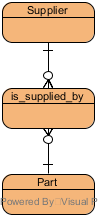
\includegraphics[scale=0.7]{img/02_many_to_many_erd.png}
				\end{flushright}
		\end{columns}
	\end{frame}
	
	\subsection{Advanced Example of Entity-Relationship Diagram}
	\begin{frame}{Advanced Example of Entity-Relationship Diagram}
	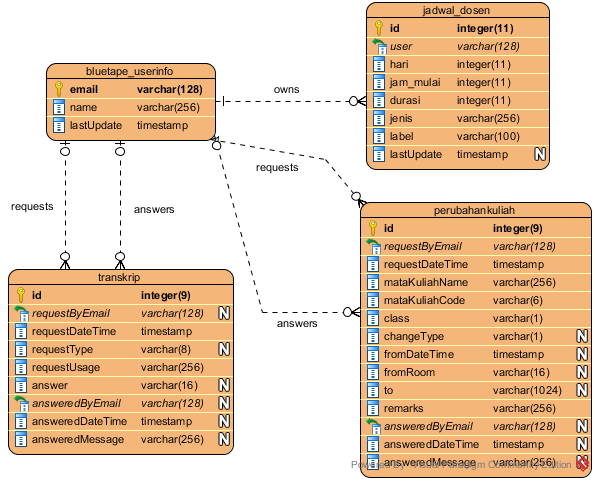
\includegraphics[scale=0.4]{img/02_bluetape.png}
    	\begin{itemize}
    	    \item Website at \url{https://bluetape.azurewebsites.net}
    	    \item Source at \url{https://github.com/ftisunpar/BlueTape}
    	\end{itemize}
	\end{frame}	
	
	\section{References}
	\begin{frame}[allowframebreaks]
        \frametitle{References}
        \bibliographystyle{amsalpha}
        \bibliography{module_02}
	\end{frame}	
\end{document}

